%%
%% This is file `test-spacing.tex',
%% generated with the docstrip utility.
%%
%% The original source files were:
%%
%% phd.dtx  (with options: `test-spacing')
%% ----------------------------------------------------------------
%% phd --- A package to beautify documents.
%% E-mail: yannislaz@gmail.com
%% Released under the LaTeX Project Public License v1.3c or later
%% See http://www.latex-project.org/lppl.txt
%% ----------------------------------------------------------------
%% 
\documentclass{ltxdoc}
\usepackage[a4paper,left=2.25cm,right=2.25cm,top=2.5cm,
            bottom=2.5cm]{geometry}
\usepackage{phd}

\cxset{style13/.style={
 name=CHAPTER,
 chapter toc=true,
 chapter spaceout = none,
 chapter numbering=arabic,
 chapter after={\vskip0pt\par},
 number font-size= HUGE,
 number font-family= sffamily,
 number font-weight= bfseries,
 title font-shape= upshape,
 number color= gray!50,
 number before=\par\vspace*{5pt}\hfill\hfill,
 number dot=,
 number after={\hspace*{7pt}\par},
 number position=rightname,
 chapter font-family= sffamily,
 chapter font-weight= bold,
 chapter font-size= LARGE,
 chapter before={\thinrule\vspace*{20pt}\par\hfill\hfill},
 chapter color= black!50,
 title beforeskip={\vspace*{10pt}},
 title afterskip={\vspace*{50pt}\par},
 title before={\hfill\hfill\raggedleft},
 title after=\par\thinrule,
 title font-family= sffamily,
 title font-color= teal,
 title font-weight= bfseries,
 title font-size= huge,
 section indent=-1em,
 section align= left,
 section numbering= arabic,
 section indent=0pt,
 section beforeskip=0pt,
 section afterskip= 10pt,
 section color=teal,
 subsection align= ,
 subsection font-family= sffamily,
 subsection font-weight= bfseries,
 subsection color = teal,
 subsection font-size= large,
 subsection font-shape=,
 subparagraph number after=,
 subsubsection align=,
 blank page text=,
 chapter opening=any,
}
}

\usepackage{lipsum}
\begin{document}
\cxset{style13}
\chapter{Petri Dishes Library}

The package defines a style for drawing places of Petri nets. 

\begin{stylekey}{/tikz/place}
  This style indicates that a node is a place of a Petri net. Usually,
  the text of the node should be empty since places do not contain any
  text. You should use the |label| option to add text outside the node
  like its name or its capacity. You should use the |tokens| options,
  explained in Section~\ref{section-tokens}, to add tokens inside the
  place.
  
\begin{codeexample}[]
\begin{tikzpicture}
  \node[place,label=above:$p_1$,tokens=2]        (p1) {};
  \node[place,label=below:$p_2\ge1$,right=of p1] (p2) {};
\end{tikzpicture}
\end{codeexample}
  
  \begin{stylekey}{/tikz/every place}
    This stype is envoked by the style |place|. To change the
    appearance of places, you can change this style.
\begin{codeexample}[]
\begin{tikzpicture}
  [every place/.style={draw=blue,fill=blue!20,thick,minimum size=9mm}]
  \node[place,tokens=7,label=above:$p_1$]  (p1) {};
  \node[place,structured tokens={3,2,9},
        label=below:$p_2\ge1$,right=of p1] (p2) {};
\end{tikzpicture}
\end{codeexample}
  \end{stylekey}
\end{stylekey}
\cxset{chapter opening=any}
\makeatletter
\cxset{
 chapter opening=right,
 chapter toc=false,
 name=CHAPTER,
 numbering= WORDS, %WORDS gives errors
 number font-size=huge,
 number font-family=sffamily,
 number font-weight=bfseries,
 number before=\kern1em,
 number dot=,
 number after=,
 number position=rightname,
 % set chapter fonts 
 chapter font-family=sffamily,
 chapter font-weight=bfseries,
 chapter font-size=huge,
 chapter margin top=5cm,
 chapter margin left=0pt,
 chapter before=\par\hfill,
 chapter after=,
 chapter color=black,
 chapter spaceout=none,
 chapter title align=center,
 chapter afterindent=true,
 number color=black,
% chapter titles
 title margin top=30pt,
 title margin bottom=30pt,
 chapter title width=\textwidth,
 chapter title text-align=center,
 title font-family=sffamily,
 title font-color=black,
 title font-weight=bfseries,
 title font-size=huge,
 title font-shape=upshape,
 title before=,
 title after=,
% sections 
 section font-size=LARGE,
 section font-weight=normalfont,
 section font-family=sffamily,
 section color=black,
 section align=centering,
 section numbering=none,
 section indent=-1em,
 section beforeskip=20pt,
 section afterskip=10pt,
 section spaceout=soul,
 section font-shape=,
 pagestyle = plain,
 subsection color=black,
}

\chapter{Introduction to Style 10}

\addcontentsline{toc}{section}{Template 10 (style10)}

This style is very similar to the |verso chapter| style. I have reproduced it as close as possible to the book that gave me the inspiration titled \emph{Mind Machines}.

\begin{figure}[htb]
\centering
\fboxrule1pt
\fbox{\includegraphics[width=0.8\textwidth]{./chapters/chapter10}}
\caption{Style ten example.}
\end{figure}

Another interesting aspect is that subsections are centered and have a colon at the end of the subsection title. The setting for this is the option \lstinline{numeric=WORDS}. Use either a capital for uppercase or \lstinline{numeric=words} for lowercase number labels.

\cxset{chapter toc=true,
          chapter margin top=0pt}
\makeatother

\cxset{chapter opening=any}
\input{test-pgf-manual-01}

\chapter{Plotting
}
\pgfplotsset{
tick label style={font=\small},
label style={font={\small\sffamily}},
legend style={font={\footnotesize\sffamily}}
}
\begin{codeexample}[]
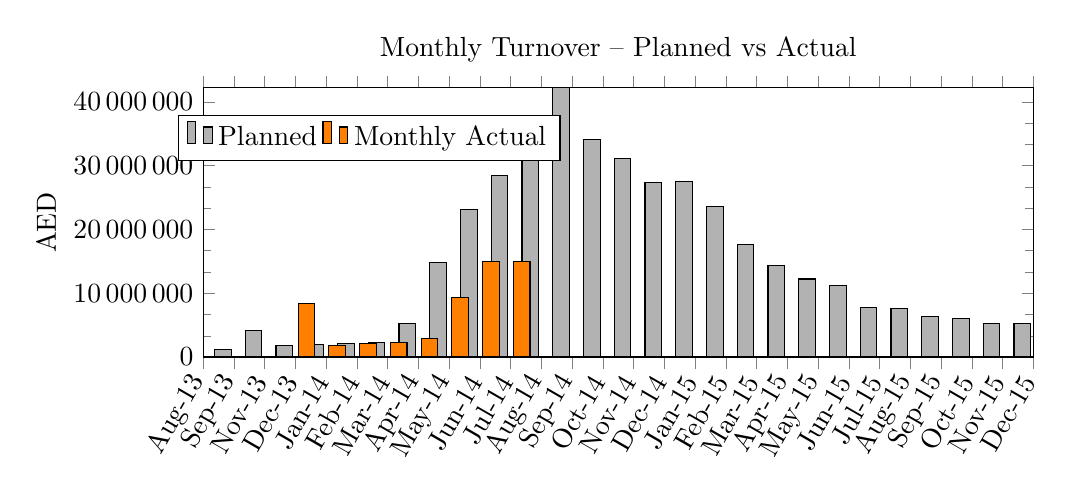
\begin{tikzpicture}
\begin{axis}[
   title={Monthly Turnover -- Planned vs Actual},
   width=1\textwidth,
   height=5cm,
   bar width=6pt,
   minor y tick num=2,
   xmajorgrids = false,
   yminorgrids=false,
   ylabel shift= -.5,
	ybar,
	enlargelimits=0.0,
	legend style={at={(0.2,0.9)},anchor=north,
	anchor=north,legend columns=-1},
	ylabel={AED},
   ytick = {0,10000000,20000000,30000000,40000000},
   scaled ticks = false,
   y tick label style={
        /pgf/number format/.cd,
            1000 sep={\,},
            fixed,
            fixed zerofill,
            precision=0,
                   /tikz/.cd
    },
	symbolic x coords={Aug-13,Sep-13,Nov-13,Dec-13,
                      Jan-14,Feb-14,Mar-14,Apr-14,
                      May-14,Jun-14,Jul-14,Aug-14,
                      Sep-14,Oct-14,Nov-14,Dec-14,
                      Jan-15,Feb-15,Mar-15,Apr-15,
                      May-15,Jun-15,Jul-15,Aug-15,
                      Sep-15,Oct-15,Nov-15,Dec-15},
	xtick = data,
   x tick label style={rotate=60,anchor=east},
   ] 
	%nodes near coords,
	nodes near coords align={vertical},
]
\addplot[fill=black!30] coordinates {(Aug-13, 29275) 
                      (Sep-13, 1118506) 
                      (Nov-13, 4118404) 
                      (Dec-13, 1744492)
                      (Jan-14, 1929106)
                      (Feb-14, 2071614)
                      (Mar-14, 2291612)
                      (Apr-14, 5280597)
                      (May-14, 14826470)
                      (Jun-14, 23178070)
                      (Jul-14, 28436550)
                      (Aug-14, 34928860)
                      (Sep-14, 42203710)
                      (Oct-14, 34092590)
                      (Nov-14, 31064640)
                      (Dec-14, 27368860)
                      (Jan-15, 27539670)
                      (Feb-15, 23631860)
                      (Mar-15, 17713270)
                      (Apr-15, 14334710)
                      (May-15, 12238960)
                      (Jun-15, 11169200)
                      (Jul-15, 7822311)
                      (Aug-15, 7654239)
                      (Sep-15, 6298405)
                      (Oct-15,6069190)
                      (Nov-15,5292039)
                      (Dec-15,5310467) 
         };
\addplot[fill=orange] coordinates {(Aug-13, 0) 
                      (Sep-13, 0) 
                      (Nov-13, 0)
                      (Dec-13, 8330874)
                      (Jan-14, 1835372) 
                      (Feb-14, 2116680)
                      (Mar-14, 2284853)
                      (Apr-14, 2860646)
                      (May-14, 9301770) 
                      (Jun-14, 15000000)
                      (Jul-14, 15000000)
};

\legend{Planned, Monthly Actual}
\end{axis}
\end{tikzpicture}
\label{barchart}
\end{codeexample}

\kant[1]
\end{document}

\endinput
%%
%% End of file `test-spacing.tex'.
